\documentclass[../main.tex]{subfiles}

\begin{document}
	
	\chapter{代码主体结构}
	\vspace{-2cm}
	
	在本章节中,我们将对BasicSR代码框架进行一个整体介绍,主要包括以下内容:整体框架、配置与注册器、数据、网络结构、模型、损失函数、训练、算子等。通过阅读本章,你将对BasicSR有进一步的认识,理解其模块之间的相互关系、以及模块内部的核心工作原理。
	
	%##################################################################################################
	%\begin{figure}[htbp]
	%	\begin{center}
	%		
\includegraphics[width=\linewidth]{figures/basicsr_logo.png}
	%		\vspace{-1cm}
	%		\caption{图标题。BasicSR Logo。}
	%		\label{fig:logo}
	%	\end{center}
	%\end{figure}
	%##################################################################################################
	
	\section{整体框架}
	对于基于深度学习的算法框架,其核心的组成部分包括:数据、模型结构、损失函数、训练策略。BasicSR框架也是大致根据以上部分撰写而成的。下图概括了BasicSR的整体组成框架:
	
	\begin{figure}[htbp]
		\begin{center}
			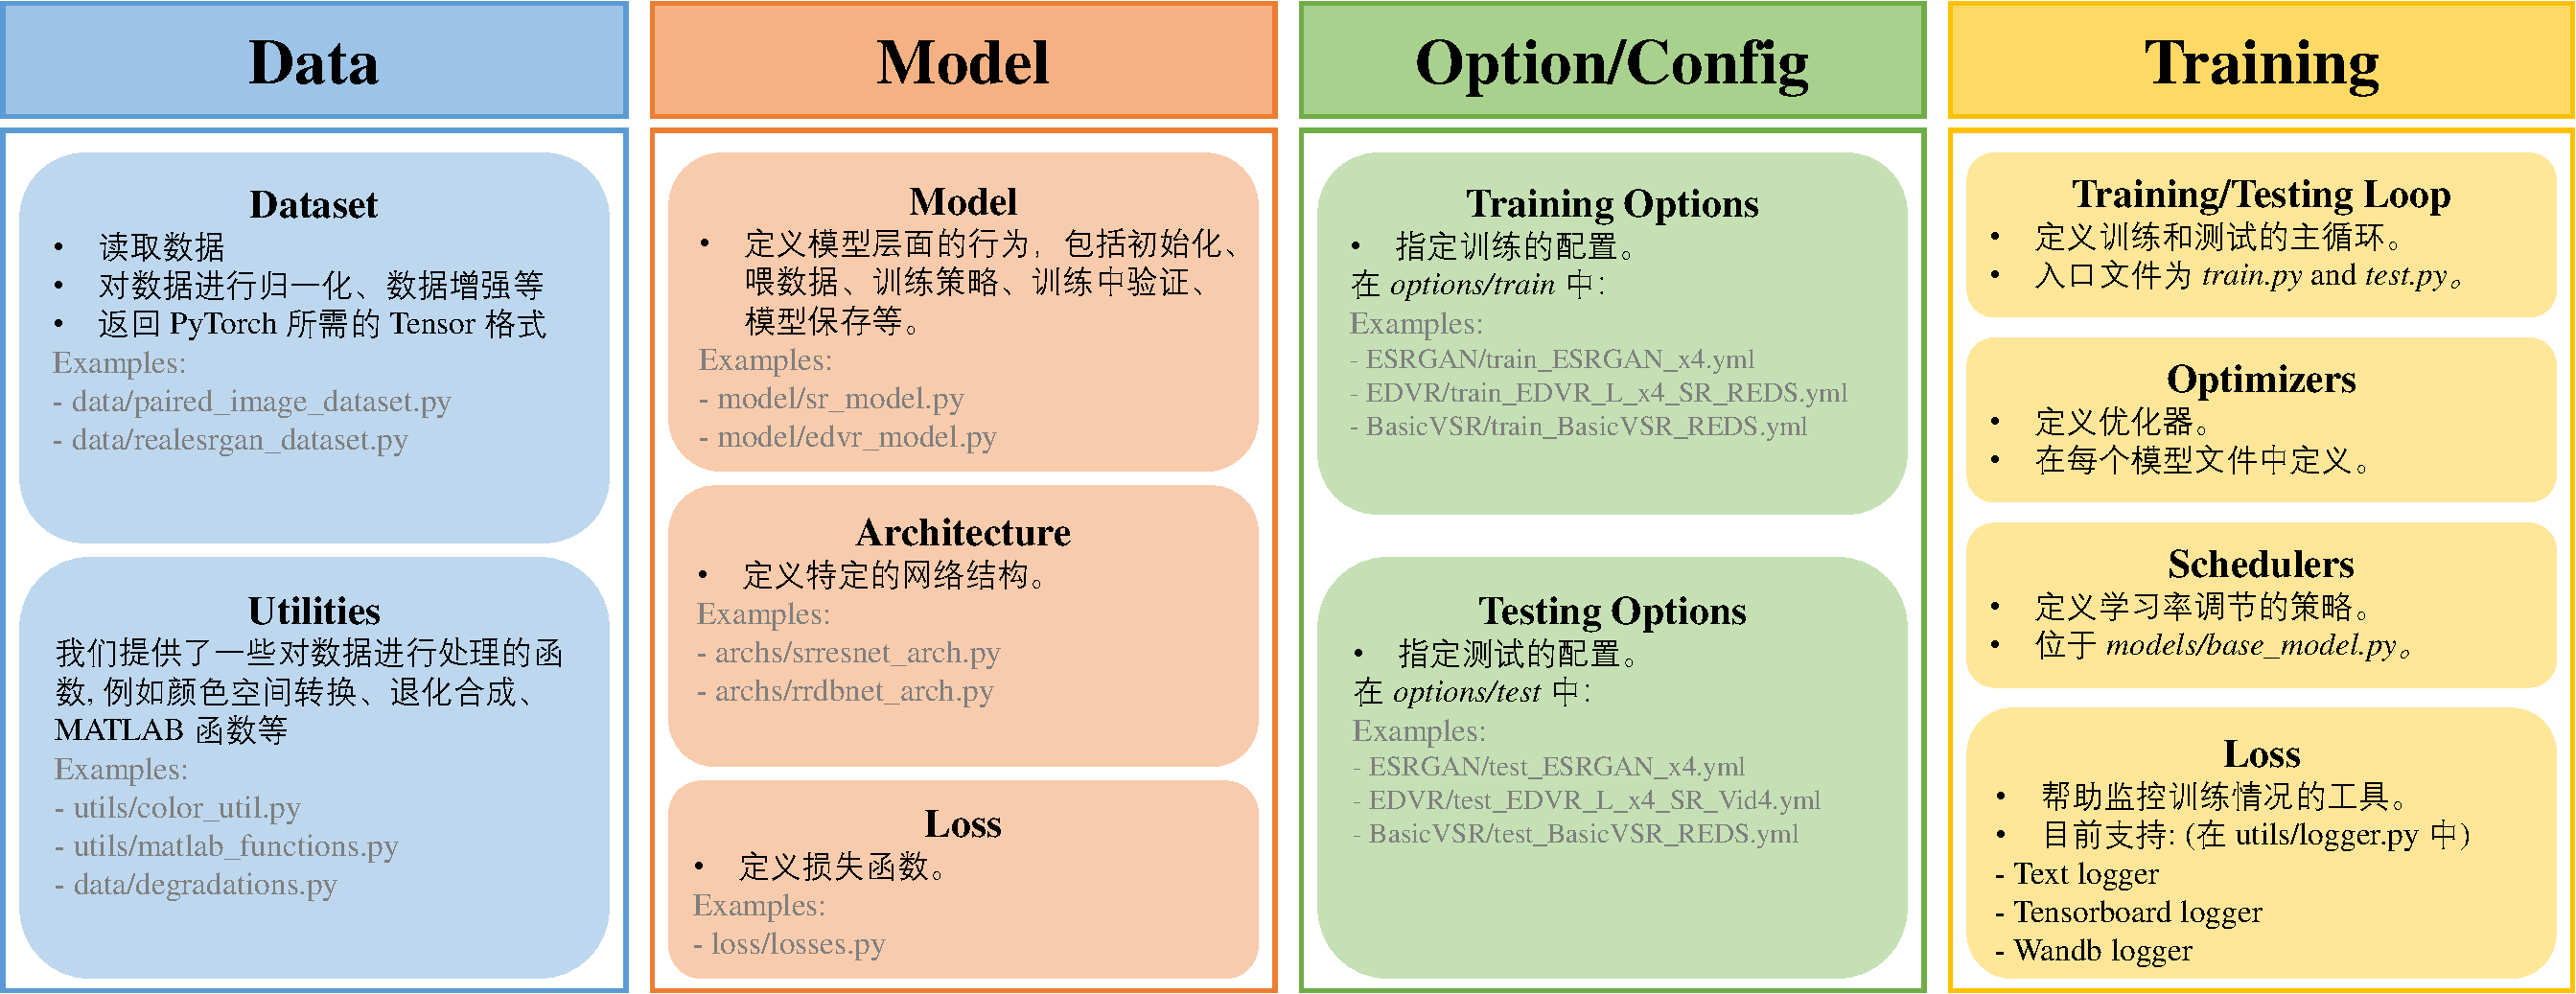
\includegraphics[width=1\linewidth]{figures/main_framework.pdf}
		\end{center}
		\caption{BasicSR代码整体框架}
		\label{fig:main_framework}
		
	\end{figure}
	
	- 数据(Data):这个部分主要定义了Dataset文件。Dataset用于读取和预处理数据,包括图像读取、归一化(normalization)、简单的数据增强(augmentation)以及封装为PyTorch Tensor等。同时,我们也提供了一些辅助函数,帮助使用者自定义自己的数据预处理功能,例如图像色彩空间转换、常用MATLAB的Python版本、常用的图像退化模型(degradation model)等。
	
	- 模型(Model):在models目录下,我们提供了常用的模型文件。这些模型文件主要用于定义数据流、训练策略、网络初始化等。在archs目录下,我们提供了常用的网络结构模型文件,包括SRResNet、RRDBNet、RCAN、SwinIR、BasicVSR等。在losses/losses.py文件中,我们提供了常用的图像复原损失函数,例如L1/L2 loss、perceptual loss、GAN loss等。
	
	- 配置(Option):在option目录下,我们提供了常用模型的训练和测试配置文件,修改这些yml文件可以简易地调整网络结构的深度、指定训练参数等。
	
	- 训练(Training):这一部分主要涉及训练的策略和记录训练日志。train.py和test.py是启动模型训练和测试的入口文件,其中定义了main loop。优化器(optimizer)的定义在各自的模型文件中可以找到。学习率的调度策略在models/base\_model.py中定义。为了方便追踪记录训练的过程,我们提供了相应的logger工具,支持直接打印、Tensorboard、Wandb等方式,具体代码可以在utils/logger.py中找到。
	
	
	- 详细的代码接口文档可以在 \url{http://basicsr.readthedocs.io}查询。
	
	
	
	\section{配置(Options)与注册器(Register)}
	\subsection{配置文件简要说明}
	- 训练的配置文件在options/train中,测试的配置文件在options/test中。通过option文件,我们可以设置实验名、选择模型文件、指定GPU、指定数据路径、选择网络结构、配置训练策略等。
	
	- 我们以train\_MSRResNet\_x4.yml为例,简单说明配置文件的每个部分。
	
	\begin{minted}[xleftmargin=1pt,bgcolor=bg]{python}
    # general settings
    name: 001_MSRResNet_x4_f64b16_DIV2K_1000k_B16G1_wandb
    model_type: SRModel
    scale: 4
    num_gpu: 1  # set num_gpu: 0 for cpu mode
    manual_seed: 0
	\end{minted}
	\begin{exampleBox}[righthand ratio=0.00, sidebyside, sidebyside align=center, lower separated=false]{一般性配置}
	
	name:自定义的实验名称。
	
    model\_type:选择模型,如SRModel,SRGANModel,EDVRModel等。
    
    scale:超分上采样尺度(upscale factor)。
    
    num\_gpu:指定GPU。
    
    manual\_seed:指定随机种子。
    \end{exampleBox}
    
	\begin{minted}[xleftmargin=1pt,bgcolor=bg]{python}
    # dataset and data loader settings
    datasets:
      train:
        name: DIV2K
        type: PairedImageDataset
        dataroot_gt: datasets/DF2K/DIV2K_train_HR_sub
        dataroot_lq: datasets/DF2K/DIV2K_train_LR_bicubic_X4_sub
        meta_info_file: basicsr/data/meta_info/meta_info_DIV2K800sub_GT.txt
        # (for lmdb)
        # dataroot_gt: datasets/DIV2K/DIV2K_train_HR_sub.lmdb
        # dataroot_lq: datasets/DIV2K/DIV2K_train_LR_bicubic_X4_sub.lmdb
        filename_tmpl: '{}'
        io_backend:
          type: disk
          # (for lmdb)
          # type: lmdb
        
        gt_size: 128
        use_hflip: true
        use_rot: true
    
        # data loader
        use_shuffle: true
        num_worker_per_gpu: 6
        batch_size_per_gpu: 16
        dataset_enlarge_ratio: 100
        prefetch_mode: ~
	\end{minted}
	\begin{exampleBox}[righthand ratio=0.00, sidebyside, sidebyside align=center, lower separated=false]{数据读取相关配置}
	
	name:自定义的数据集名称。
	
	type:读取数据的Dataset类,例如PairedImageDataset等。详细请查看《模型》部分。
	
	dataroot\_gt:ground-truth图像存放的目录。
	
	dataroot\_lq:input图像存放的目录。
	
	meta\_info\_file:预先生成的meta\_info文件。细节请查看《数据准备》章节。
	
	gt\_size:训练阶段,crop的ground truth图像的尺寸大小,即label大小。
	
	use\_hflip:是否开启水平方向图像增强(随机水平翻转图像)。
	
	use\_rot:是否开启旋转图像增强(随机旋转图像)。
	
	use\_shuffle:训练时是否随机打乱数据顺序。
	
	num\_worker\_per\_gpu:每块GPU分配的线程数。
	
	batch\_size\_per\_gpu: 每块GPU分配的batch size。
	
	dataset\_enlarge\_ratio: xxx
    
    prefetch\_mode: xxx
    
    \end{exampleBox}
    
    \begin{minted}[xleftmargin=1pt,bgcolor=bg]{python}
    val:
        name: Set5
        type: PairedImageDataset
        dataroot_gt: datasets/Set5/GTmod12
        dataroot_lq: datasets/Set5/LRbicx4
        io_backend:
          type: disk
    
      val_2:
        name: Set14
        type: PairedImageDataset
        dataroot_gt: datasets/Set14/GTmod12
        dataroot_lq: datasets/Set14/LRbicx4
        io_backend:
          type: disk
	\end{minted}
	\begin{exampleBox}[righthand ratio=0.00, sidebyside, sidebyside align=center, lower separated=false]{validation配置}
	
	val部分为训练时validation的数据配置。通过定期validation,我们可以及时观察训练的情况,追踪模型当前的表现。
    \end{exampleBox}
    \begin{minted}[xleftmargin=1pt,bgcolor=bg]{python}
    # network structures
    network_g:
      type: MSRResNet
      num_in_ch: 3
      num_out_ch: 3
      num_feat: 64
      num_block: 16
      upscale: 4
	\end{minted}
	\begin{exampleBox}[righthand ratio=0.00, sidebyside, sidebyside align=center, lower separated=false]{网络结构相关配置}
	
	type:选择网络结构模型,例如MSRResNet,RRDBNet等。
	
	num\_in\_ch:模型输入的图像通道数。
	
	numx\_out\_ch: 模型输出的图像通道数。
    
    num\_feat: 模型内部的feature map通道数。
    
    num\_block: 模型内部基础模块的堆叠数。
    
    upscale: 上采样倍数。
    \end{exampleBox}
    \begin{minted}[xleftmargin=1pt,bgcolor=bg]{python}
    # path
    path:
      pretrain_network_g: ~
      strict_load_g: true
      resume_state: ~
	\end{minted}
	\begin{exampleBox}[righthand ratio=0.00, sidebyside, sidebyside align=center, lower separated=false]{模型存储路径相关配置}
	
	pretrain\_network\_g: 测试或者finetune时,在在这里输入保存的模型权重路径。
	
    strict\_load\_g: 是否根据参数名称一一对应严格load模型参数。
    
    resume\_state: 如训练被打断,可以在这里填写保存的状态文件,恢复训练。
    \end{exampleBox}
    \begin{minted}[xleftmargin=1pt,bgcolor=bg]{python}
    # training settings
    train:
      ema_decay: 0.999
      optim_g:
        type: Adam
        lr: !!float 2e-4
        weight_decay: 0
        betas: [0.9, 0.99]
    
      scheduler:
        type: CosineAnnealingRestartLR
        periods: [250000, 250000, 250000, 250000]
        restart_weights: [1, 1, 1, 1]
        eta_min: !!float 1e-7
    
      total_iter: 1000000
      warmup_iter: -1  # no warm up
    
      # losses
      pixel_opt:
        type: L1Loss
        loss_weight: 1.0
        reduction: mean
	\end{minted}
	\begin{exampleBox}[righthand ratio=0.00, sidebyside, sidebyside align=center, lower separated=false]{训练策略相关配置}
	
	ema\_decay:EMA参数更新权重。
	
	optim\_g type: 选择优化器,例如Adam。
	
    lr: 初始学习率。
    
    weight\_decay: 权重衰退参数。
    
    betas: 优化器动量参数。
	
    scheduler type: 选择学习率更新策略,例如CosineAnnealingRestartLR。
    
    periods: 学习率更新周期。
    
    restart\_weights: 如果选择学习率restart机制,在这里可以指定restart时的权重。
    
    eta\_min: 学习率衰退的最小值。
    
    total\_iter: 总共进行的训练迭代次数。
    
    warmup\_iter: warm up的迭代次数。
    
    pixel\_opt type: 选择loss函数,例如L1Loss。
    
    loss\_weight: 指定loss的权重。
    
    reduction: 计算loss取平均或者总和。
    
    \end{exampleBox}
    \begin{minted}[xleftmargin=1pt,bgcolor=bg]{python}
    # validation settings
    val:
      val_freq: !!float 5e3
      save_img: false
    
      metrics:
        psnr: # metric name, can be arbitrary
          type: calculate_psnr
          crop_border: 4
          test_y_channel: false
          better: higher  # the higher, the better. Default: higher
        niqe:
          type: calculate_niqe
          crop_border: 4
          better: lower  # the lower, the better
	\end{minted}
	\begin{exampleBox}[righthand ratio=0.00, sidebyside, sidebyside align=center, lower separated=false]{validation相关配置}
	
	val\_freq: 多少次迭代进行一次validation。
	
    save\_img: 是否保存validation的图像。
    
    metrics:validation时的指标设定。
    
    type: 选择指标,例如calculate\_psnr,calculate\_niqe。
    
    crop\_border: 计算指标时crop图像边界像素范围。
    
    test\_y\_channel: 是否仅在Y通道上计算指标。
    
    better: 该指标是越高越好,还是越低越好。选择higher或者lower,默认为higher。
    \end{exampleBox}
    \begin{minted}[xleftmargin=1pt,bgcolor=bg]{python}
    # logging settings
    logger:
      print_freq: 100
      save_checkpoint_freq: !!float 5e3
      use_tb_logger: true
      wandb:
        project: ~
        resume_id: ~
	\end{minted}
	\begin{exampleBox}[righthand ratio=0.00, sidebyside, sidebyside align=center, lower separated=false]{训练日志相关配置}
	
	print\_freq: 多少次迭代打印一次训练信息。
    
    save\_checkpoint\_freq: 多少次迭代保存一次模型权重。
    
    use\_tb\_logger: 是否开启Tensorboard。
    \end{exampleBox}
    
    \subsection{动态实例化与REGISTER注册机制}
	\textbf{动态实例化}
	
	- 当我们新写了类(Class)或函数时,可直接在配置文件中使用。程序会根据配置文件的类名或函数名,自动查找并实例化。这个过程称为动态实例化(Dynamic Instantiation)。
	
	- 具体而言,我们是通过importlib和getattr来实现的。以data为例,我们在data/\_\_init\_\_.py 中是如下做的:

    1. 扫描所有以\_dataset.py为结尾的文件(这是约定);
    
    2. 把这些文件中的类或函数通过importlib都import进来;
    
    3. 根据配置文件中的名称,通过getattr实例化。
    
    具体操作的代码如下:(读者只需知道这个机制即可,以下代码不影响BasicSR的直接使用)
	\begin{minted}[xleftmargin=1pt,bgcolor=bg]{python}
    # automatically scan and import dataset modules
    # scan all the files under the data folder with '_dataset' in file names
    data_folder = osp.dirname(osp.abspath(__file__))
    dataset_filenames = [
        osp.splitext(osp.basename(v))[0] for v in scandir(data_folder)
        if v.endswith('_dataset.py')
    ]
    # import all the dataset modules
    _dataset_modules = [
        importlib.import_module(f'basicsr.data.{file_name}')
        for file_name in dataset_filenames
    ]
    
    ...
    
    # dynamic instantiation
    for module in _dataset_modules:
        dataset_cls = getattr(module, dataset_type, None)
        if dataset_cls is not None:
            break
	\end{minted}
	
	- 我们对以下模块使用了类似的技巧,在使用的时候需要注意文件后缀名称的约定:
	\begin{table}[h]
	\centering
    \begin{tabular}{|c|c|c|}
    \hline
    \textbf{Module} & \textbf{File Suffix} & \textbf{Example} \\ \hline
    Data & \_dataset.py & data/paired\_image\_dataset.py \\ \hline
    Model & \_model.py & basicsr/models/sr\_model.py \\ \hline
    Archs & \_arch.py & basicsr/archs/srresnet\_arch.py \\ \hline
    \end{tabular}
    \caption{动态实例化文件命名约定}
    \end{table}
    
    \begin{hl} % ---------------- Highlight block ---------------- %
	\textbf{注意}
	
	1. 上面的文件后缀只用在需要的文件中,其他文件命名尽量避免使用以上的后缀。
	
	2. 类名或函数名不能重复。
    \end{hl}
    
    - 另外,对losses和metrics,我们也使用了importlib和getattr,但是和上面不一样的是,对于losses和metrics,由于文件数量比较少,改动也少,因此我们不采用扫描文件的方式,而是在新增加类/函数后,需要在相应的\_\_init\_\_.py 中增加类/函数名称。
    \begin{table}[h]
    \centering
    \begin{tabular}{|c|c|c|}
    \hline
    \textbf{Module} & \textbf{Path} & \textbf{Modify} \\ \hline
    Losses & basicsr/models/losses & basicsr/models/losses/\_\_init\_\_.py \\ \hline
    Metrics & basicsr/metrics & basicsr/metrics/\_\_init\_\_.py \\ \hline
    Archs & \_arch.py & basicsr/archs/srresnet\_arch.py \\ \hline
    \end{tabular}
    \caption{部分类的实例化需要修改对应的\_\_init\_\_.py文件}
    \end{table}
    
    - 在Log的时候, loss项使用l\_开头,这样在Tensorboard显示的时候,所有loss会被组织到一起。比如在basicsr/models/srgan\_model.py中,使用了l\_g\_pix,l\_g\_percep,l\_g\_gan等。在basicsr/utils/logger.py中,他们会被组织到一起:
    \begin{minted}[xleftmargin=1pt,bgcolor=bg]{python}
    if k.startswith('l_'):
        self.tb_logger.add_scalar(f'losses/{k}', v, current_iter)
    else:
        self.tb_logger.add_scalar(k, v, current_iter)
	\end{minted}

	
	\begin{minted}[xleftmargin=20pt,linenos,bgcolor=bg]{python}
		class RepConv(nn.Module):
		"""Re-parameterizable block for RepSR."""
		
		def __init__(self,
		in_channels,
		out_channels,
		kernel_size,
		stride=1,
		padding=0,
		dilation=1,
		groups=1,
		padding_mode='zeros',
		deploy=False,
		width_multiplier=2,
		with_bn=True,
		frozen_bn=False):
		super(RepConv, self).__init__()
		self.deploy = deploy
		self.in_channels = in_channels
		self.out_channels = out_channels
		self.kernel_size = kernel_size
		self.stride = stride
		self.padding = padding
		self.dilation = dilation
		self.groups = groups
		self.with_bn = with_bn
		self.frozen_bn = frozen_bn
		
		self.mid_channels = out_channels * width_multiplier
		self.rep_c1_2 = nn.Conv2d(
		in_channels=self.mid_channels,
		out_channels=out_channels,
		kernel_size=1,
		stride=stride,
		padding=0,
		groups=groups,
		bias=True)
		
		# initialization
		init_list = [
		self.rep_identity, self.rep_c3_1, self.rep_c1_1, self.rep_c3_2,
		self.rep_c1_2
		]
		if with_bn:
		init_list.extend([self.rep_bn_1, self.rep_bn_2])
		default_init_weights(init_list, scale=0.1)
		
		def forward(self, inputs, frozen_bn=None):
		if frozen_bn is None:
		frozen_bn = self.frozen_bn
		
		if hasattr(self, 'rep_merge'):
		return self.rep_merge(inputs)
		if self.with_bn:
		id_out = self.rep_identity(inputs)
		out_1 = self.rep_c1_1(
		self.rep_bn_1(self.rep_c3_1(inputs), frozen_bn))
		out_2 = self.rep_c1_2(
		self.rep_bn_2(self.rep_c3_2(inputs), frozen_bn))
		else:
		id_out = self.rep_identity(inputs)
		out_1 = self.rep_c1_1(self.rep_c3_1(inputs))
		out_2 = self.rep_c1_2(self.rep_c3_2(inputs))
		
		return id_out + out_1 + out_2
	\end{minted}
	
	
	\section{数据(Data Loader)}
	
	\section{网络结构(Architecture)}
	
	\section{模型(Model)}
	
	- Base模型
	
	- 其他模型
	
	- 继承关系
	
	\section{损失函数(Loss)}
	
	\section{训练(优化器与学习率调度器)}
	
	\section{算子}
	
\end{document}